\chapter{Related Work}
\label{ch:related}

In this chapter, we focus on previous work that is related to the problem stated in \nameref{ch:introduction}. We first present a theoretical approach for creating a synchronized graphical and code editor. Next, we introduce a list of existing tools for editing RDF vocabularies (visually, textually or both). Finally, we show why visualizing semantic data can raise several problems and we explain the solutions that were found.


\section{A Synchronization Approach}

An approach which is meant to ease the work with languages that feature both textual and graphical syntax has been investigated by van Rest et al. in \cite{Rest2013}. This work also suggests ways to overcome common synchronization problems such as error recovery and layout preservation.

The main idea of the method is having two interconnected underlying models, one for each editor. While the graphical changes can be pushed directly into the corresponding model, the textual side needs an intermediary - abstract syntax trees (AST), which can be regarded as tree representations of the syntactic structure of the code. Abstract syntax trees are commonly used by compilers during semantic analysis, in order to verify that the elements of the programming language are correctly used.

\begin{figure}[!htbp]
	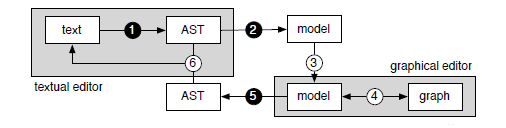
\includegraphics[width=\linewidth]{img/robust_real_time_sync.png}
	\caption{Steps involved in the synchronization process: 1) parsing, 2) tree to model transformation, 3) model merge, 4) graphical changes propagation, 5) model to text transformation, 6) tree to text printing. Figure taken from \cite{Rest2013}.}
	\label{img:robust_sync}
\end{figure}

\autoref{img:robust_sync} presents a broad overview of this approach. For the textual to graphical view synchronization, the code is parsed into an abstract syntax tree, which is then turned into a model. The resulting model is merged with the one belonging to the graphical view and then this view is updated accordingly. The inverse synchronization process starts with pushing the graphical changes into the model, followed by its transformation into an abstract syntax tree. The resulting tree is merged with the one belonging to the code view, which will be turned into text.

This approach is not completely applicable in our case as some steps do not need explicit implementation. For example, we are not bound to use abstract syntax trees, as parsing RDF data is already supported by existing frameworks, such as the \textit{N3.js} Javascript library\footnote{\url{https://github.com/RubenVerborgh/N3.js}}. Moreover, we do not have to use one model for each view. In fact, we will consider this idea but, in our case, a more feasible approach is having a centralized underlying model for both views: the textual and graphical data shall be parsed directly into the common model, followed by an update process responsible for propagating the changes to the other view.

\section{Vocabulary Editors}
\label{sec:editors}

In this section, we will present a few tools for authoring and editing RDF vocabularies. Some of them feature only textual editors with the possibility to visualize the result, while the others enable the user to also edit the graphical display. None of them, though, synchronize the changes without user interaction.

\textbf{1. IsaViz}\footnote{\url{https://www.w3.org/2001/11/IsaViz}} is a visual environment for browsing and authoring RDF models as graphs. This tool is offered by the W3C Consortium \cite{Kapoor2010}, but it has not been maintained since 2007. IsaViz comes with an user interface which allows creating and editing graphs, together with zooming and navigation into the model. However, it does not provide any clustering or other abstraction of the graph visualization, which quickly results in large RDF graphs that are hard to read and handle. \autoref{img:tools}(a) shows an example of the interface. The changes occurring in the graphical view can be synchronized with the text only through file export. The tool allows importing ontologies in formats like RDF/XML, Notation3 and N-Triple, while the export supports, besides the already mentioned formats, also SVG and PNG.

\textbf{2. Protégé}\footnote{\url{http://protege.stanford.edu}} is an ontology editor created by Stanford University and actively supported by the Protégé community. The tool allows the definition of classes, class hierarchies, variables, variable-value restrictions, relationships between classes and the properties of these relationships \cite{Kapoor2010}. Ontologies can be uploaded and downloaded in various formats such as RDF/XML, Turtle, OWL/XML and OBO. Protégé's functionality can be divided into three areas: creating ontologies, creating data using the ontology and querying the data. Moreover, the software comes with visualization packages (OntoViz\footnote{\url{http://protegewiki.stanford.edu/wiki/OntoViz}}, EZPAL\footnote{\url{http://protegewiki.stanford.edu/wiki/EZPal}} and others) and it can create a graphical user interface from the ontology, that is, forms with fields corresponding to elements in the ontology \cite{Steer2002}. An example can be viewed in \autoref{img:tools}(b). Protégé features a web extension - Web-Protégé, which aims to better support the collaborative development process in a web environment. The tool provides support for simultaneous editing, where a change made by a user is immediately seen by the other users \cite{Tudorache2008}. Both editors enable modifying the graphical view, i.e., the fields in the forms, and the changes can be exported into text files having the previously mentioned formats. This means, however, that immediate synchronization is not supported.

\textbf{3. OntoSketch} \cite{Brade2013} takes a different approach for editing ontologies: the RDF graph elements can be drawn on a tablet computer using pen and paper-like interactions (\autoref{img:tools}(c)). The sketches are then converted into RDF triples that can be exported and further edited in other tools. The editor is available only as an Android application for tablets. Although this might assist domain experts to actively participate in ontology modeling, the aforementioned limitations remain.

\textbf{4. Vocabulary collaboration and build environment} (VoCol) \cite{Halilaj2016} offers a collaborative environment for building ontologies. Vocabulary files storage and versioning control are achieved through repository services like GitHub, GitLab and BitBucket. VoCol comes with a code editor for Turtle format, where files can be loaded from the repository and be modified. The changes can be committed only when they pass certain rules of correctness, the editor featuring syntax validation, implemented with tools like Rapper\footnote{\url{http://librdf.org/raptor/rapper.html}} or Jena Riot\footnote{\url{https://jena.apache.org/documentation/io}}. Furthermore, this environment offers the possibility of visualizing vocabulary elements using WebVOWL\footnote{\url{http://vowl.visualdataweb.org/webvowl.html}}. \autoref{img:tools}(d) shows an example of the interface. The graphical view is not editable, though, and can be updated only after the changes were committed to the repository. The entire code base is open source and available on GitHub\footnote{\url{https://github.com/vocol/vocol}}. An important observation to be made at this point is that our implementation has as prerequisite the code editor offered by Vocol, together with its repository services.

Most available tools support either visualization of existing ontologies or visual creation of new ontologies, but only few tools support both. Especially a synchronized textual and visual editing approach is currently not provided by the available RDF-based ontology editing tools to the best of our knowledge.

\begin{figure}[htb]

\begin{minipage}[b]{.48\linewidth}
  \centering
  \centerline{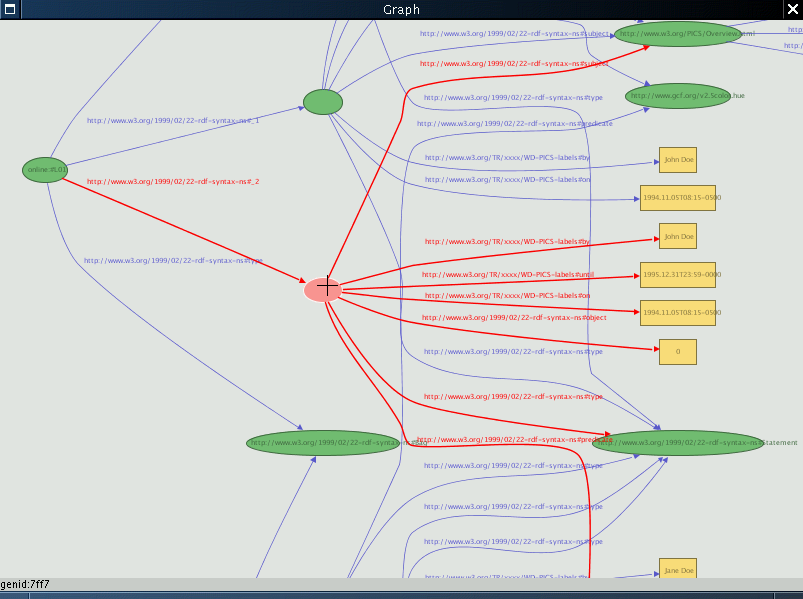
\includegraphics[width=6.7cm, height=4.7cm]{img/isaviz.png}}
%  \vspace{1.5cm}
  \centerline{(a) IsaViz}\medskip
\end{minipage}
\hfill
\begin{minipage}[b]{0.48\linewidth}
  \centering
  \centerline{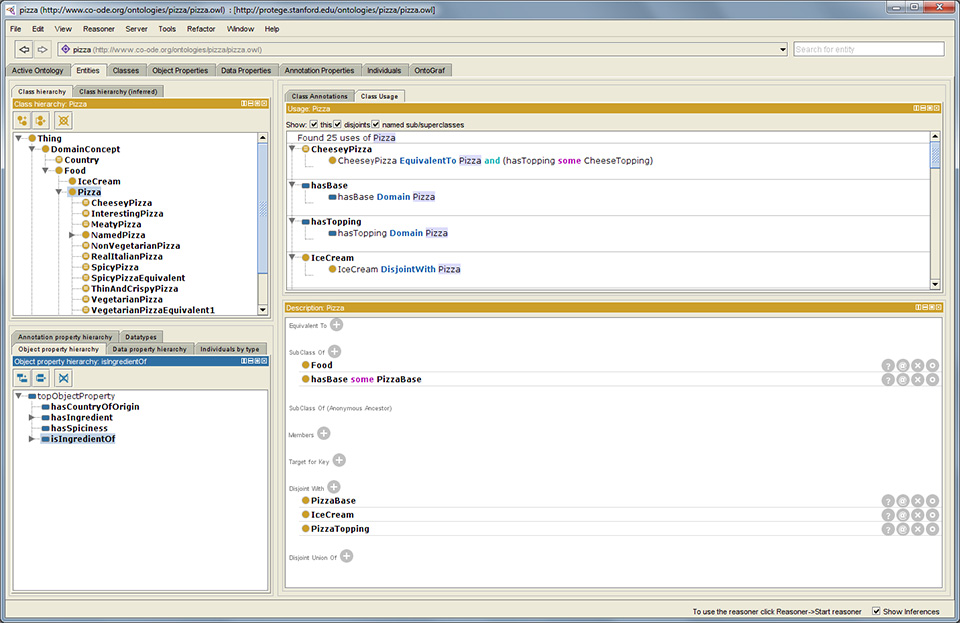
\includegraphics[width=6.7cm, height=4.7cm]{img/protege.jpg}}
%  \vspace{1.5cm}
  \centerline{(b) Protégé}\medskip
\end{minipage}
\begin{minipage}[b]{.48\linewidth}
  \centering
  \centerline{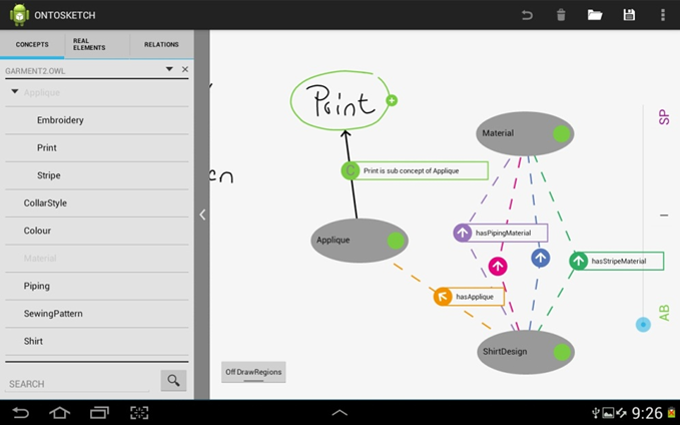
\includegraphics[width=6.7cm, height=4.7cm]{img/ontosketch.png}}
%  \vspace{1.5cm}
  \centerline{(c) OntoSketch}\medskip
\end{minipage}
\hfill
\begin{minipage}[b]{0.48\linewidth}
  \centering
  \centerline{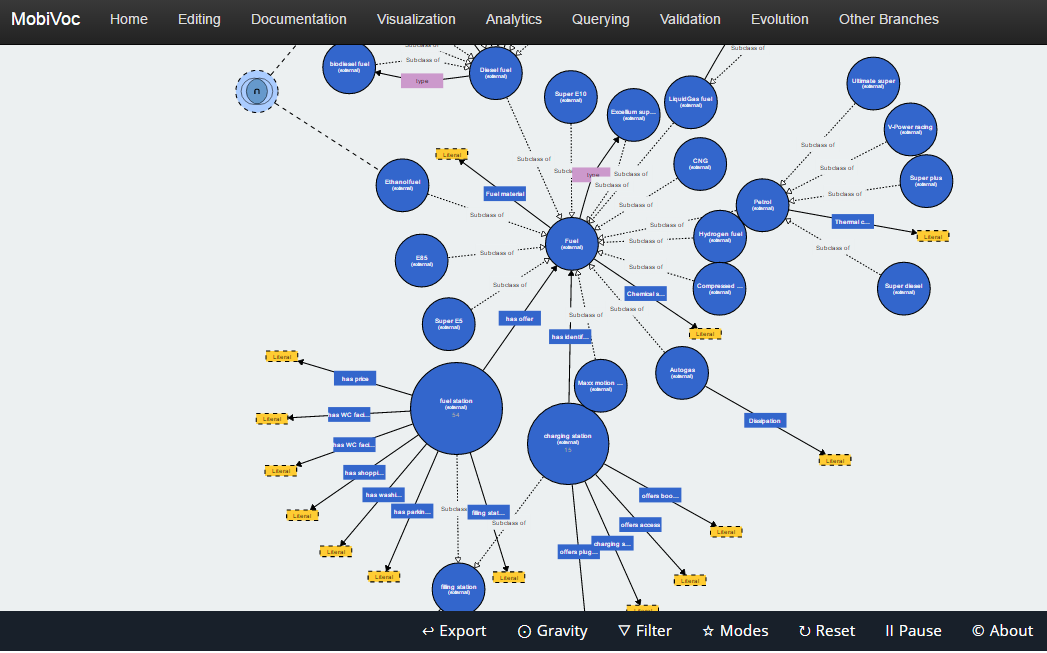
\includegraphics[width=6.7cm, height=4.7cm]{img/vocol.png}}
%  \vspace{1.5cm}
  \centerline{(d) VoCol}\medskip
\end{minipage}
%
\caption{Graphical user interfaces of different tools for editing RDF vocabularies.}
\label{img:tools}
%
\end{figure}


\section{Visualizing Semantic Data}
\label{sec:visualizing_semantic_data}

RDF data visualization tools are usually optimized for small models. However, semantic data describing web resources can easily reach thousands of nodes and, at this point, special techniques are needed in order to display the RDF model in such a manner that it is easy to understand and navigate.

GViz \cite{Telea2002} is a general purpose visual environment for browsing and editing graph-based data. Its main advantage, compared to most other graph visualization tools, is that it is easily customizable \cite{Telea2003}. Modifying the graph layout is highly flexible, the users being able to choose the shape, color, size and other attributes of the nodes and edges. One interesting feature is the possibility to define callbacks in the Tcl scripting language\footnote{\url{https://www.tcl.tk}}, in order to further customize nodes and edges depending on certain attributes. 

\begin{figure}[!htbp]
	\centering
 	\centerline{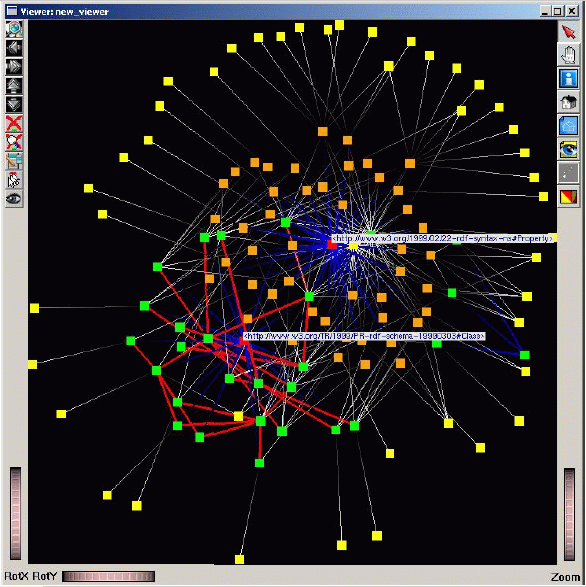
\includegraphics[width=0.7\linewidth]{img/gviz.png}}
	\caption{GViz ontology visualization. Figure taken from \cite{Telea2003}.}
	\label{img:gviz}
\end{figure}

\autoref{img:gviz} presents a visualization example, where choosing different colors makes the navigation more intuitive. Literals are depicted with yellow and displayed at the periphery as they are loose coupled, resources are green and nodes having an edge with the \textit{rdf:Property} value are displayed in orange. Edges are also differentiated through colors, depending on their value: \textit{rdf:type} is blue, \textit{rdfs:subClassOf} is red and the rest are white. Another customization is not displaying the edges as arrows, but as lines fading towards the subject, in order to avoid the clutter produced by highly connected graphs. This approach proves itself very helpful when it comes to easily finding the interesting nodes, i.e. the nodes describing the web resources that the model defines, as they will always stand out due to their different color.

Another approach for intuitive graph visualization was investigated in \cite{Mutton2003}. This method uses the properties between instances in order to place the related nodes near to each other, while keeping the other nodes evenly distributed. The resulting graph will give the user insight into the structure and relationships in the data model that are hard to see in text \cite{Mutton2003}. The drawing algorithm uses the spring embedding method \cite{Fruchterman1991}, which distributes the nodes in a two-dimensional space and, at the same time, keeps the connected nodes reasonably close together. The graph is considered a force system where each node simulates a charged particle, which causes a repulsive force, and each edge is modeled as a spring that exerts an attractive force between the pair of nodes it connects. \autoref{img:spring} shows an example of such layout where connected nodes are close together, yet no pair of nodes are too close to each other due to the repulsive forces acting between them \cite{Mutton2003}.

\begin{figure}[!htbp]
	\centering
  	\centerline{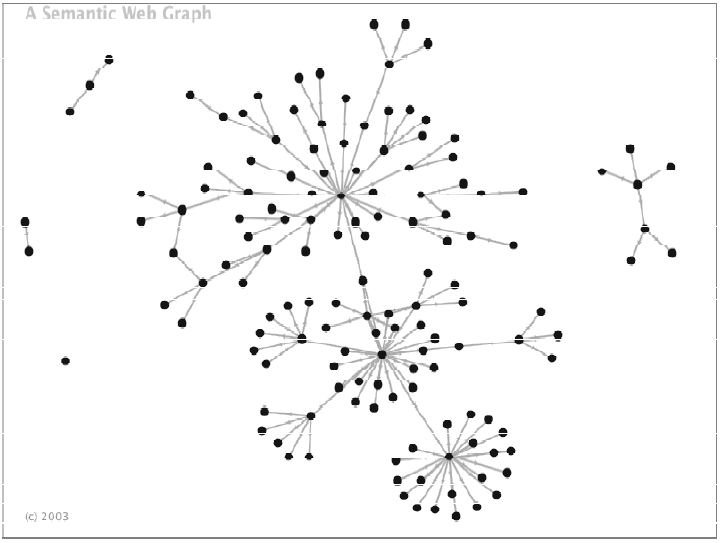
\includegraphics[width=0.7\linewidth]{img/spring.png}}
	\caption{Graph layout using spring embedding. Figure taken from \cite{Mutton2003}.}
	\label{img:spring}
\end{figure}














